\documentclass[10pt]{beamer}

\usetheme{metropolis}
\usepackage{appendixnumberbeamer}

\usepackage{booktabs}
\usepackage[scale=2]{ccicons}

\usepackage{pgfplots}
\usepgfplotslibrary{dateplot}

\usepackage{graphics}

\usepackage{xspace}
\newcommand{\themename}{\textbf{\textsc{metropolis}}\xspace}
\setbeamertemplate{frame footer}{ME738 - Special Topics in Materials}

\title{Chip Scale Atomic Clocks Sources}
\subtitle{Motivations}
\date{March 5, 2024}
\author{Tommaso Bocchietti}
\institute{University of Waterloo}
\titlegraphic{\hfill
\includegraphics[height=1.5cm]{pdf/UniversityOfWaterloo_logo_horiz_pms.pdf}}

\begin{document}

\maketitle

\begin{frame}[fragile]{Source Types}
    In the following table are reported the main types of clock sources that are based on atomic physics.
    \begin{table}

        % \resizebox{\columnwidth}{!}{%
        %     \begin{tabular}{lccc}
        %         \toprule
        %         \textbf{Parameter}      & \textbf{TCXO \cite{TCXO-VT840}} & \textbf{CSAC \cite{CSAC-SA65}}                  & \textbf{Optical CSAC} \\
        %         \midrule
        %         Power Input (mW)        & $<10mW$                         & $<120mW$                                        & 100-500               \\
        %         Operating Temperature   & $-40^oC to +85^oC$              & $-40^oC to +80^oC$                              & Room temp to 85°C     \\
        %         Temperature Sensitivity & $\pm 2 \times 10^{-6}$          & $\pm 3 \times 10^{-10}$                         & <0.001 ppm/°C         \\
        %         Startup Time (sec)      & $2ms$                           & $<180s$                                         & 1-10                  \\
        %         Aging (ppb/year)        & $<1\times10^{-6}/year$          & $<9\times10^{-10}/month | <1\times10^{-8}/year$ & <1                    \\
        %         % Drift (ppb/year)        & 500-2000                        & $3\times10^{-10}@\tau=1$                        & <1                    \\
        %         \bottomrule
        %     \end{tabular}
        % }

        \resizebox{\columnwidth}{!}{%
            \begin{tabular}{l|cccccc}
                \toprule
                \textbf{Model}                            & \textbf{Transition} & \textbf{Species} & \textbf{Drift ($\tau=1$)} & \textbf{Aging}        & \textbf{Power (mW)} & \textbf{Size (cm$^3$)} \\
                \midrule
                Microsemi SA.45s \cite{Microsemi-SA.45s}  & Microwave           & Cs               & $3\times10^{-10}$         & $<9\times10^{-10}/mo$ & $120$               & $17$                   \\
                Microsemi MAC SA.5X \cite{Microsemi-SA5X} & Microwave           & Rb               & $3\times10^{-11}$         & $<5\times10^{-11}/mo$ & $6300$              & $47$                   \\
                NIST (experimental)                       & Optical             & Rb               & $\approx10^{-13}$         & Still unknowable      & $420$               & $35$                   \\
                \bottomrule
            \end{tabular}
        }
        \caption{Comparison of clock sources}

    \end{table}

    It's clear how compared to the traditional MEMS resonator, the atomic clock sources have a much better performance in terms of both drift and aging.
    Temperature sensitivity is also much lower, but the size and cost are higher.

\end{frame}



\begin{frame}{Applications}

    In terms of applications, chip-scale optical atomic clocks are still in the experimental phase, while microwave atomic clocks are already used in commercial applications due to their lower cost, size and power consumption (battery-operated devices).

    The most important applications are related to \textbf{GNSS and GPS systems}.
    A high-precision synchronization between the satellites then permit a more reliable and accurate network synchronization on the ground.
    This open the door to a wide range of applications where a precise timing (or positioning) is required, such as:

    \begin{itemize}
        \item Defense applications (i.e. UAVs)
        \item Airline navigation (i.e. GPS-based landing systems)
        \item Cellphone telecommunications (next generation 5G networks)
        \item Financial transactions (i.e. high-frequency trading)
    \end{itemize}

\end{frame}



\begin{frame}{Outline}

    Next phases of the project will be focused on the following points:

\end{frame}



\appendix

\begin{frame}[standout]
    Notes slides
\end{frame}



\begin{frame}{Rubidium (Rb) \& Cesium (Cs)}

    \begin{columns}

        \column{0.5\textwidth}
        \begin{figure}
            \centering
            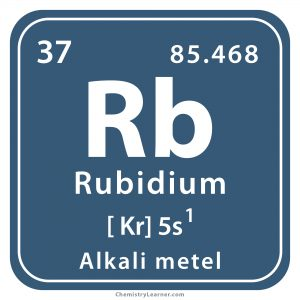
\includegraphics[width=0.3\textwidth]{img/Rubidium-Symbol}
        \end{figure}

        \column{0.5\textwidth}
        \begin{figure}
            \centering
            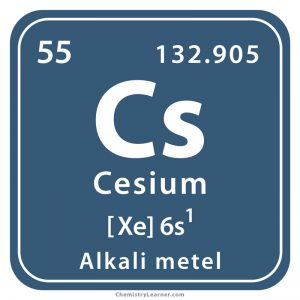
\includegraphics[width=0.3\textwidth]{img/Cesium-Symbol}
        \end{figure}

    \end{columns}

    \begin{figure}
        \centering
        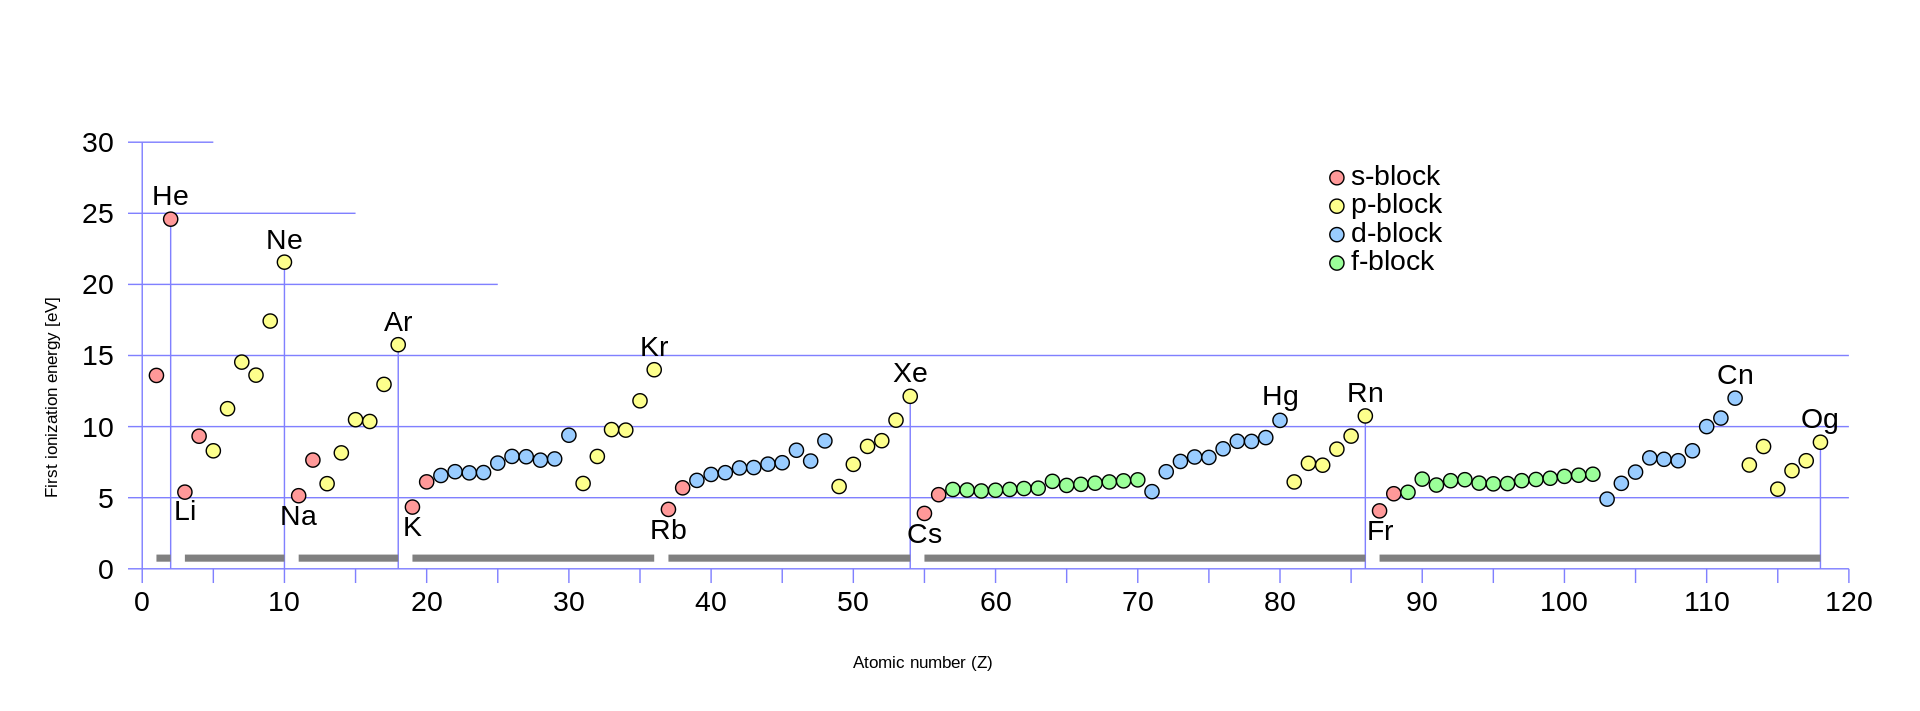
\includegraphics[width=0.9\textwidth]{img/First_Ionization_Energy}
        \caption{First ionization energy of all the elements \url{https://en.wikipedia.org/wiki/Alkali_metal}}
    \end{figure}

\end{frame}



\begin{frame}[fragile]{Drift}
    \begin{itemize}
        \item Drift refers to the gradual change in a clock's frequency over a short period of time.
        \item It can be caused by factors such as changes in temperature, mechanical stresses, or other environmental influences.
        \item Is usually observed over hours, days, or weeks, and it describes how the clock's frequency changes during these relatively short intervals.
    \end{itemize}
\end{frame}



\begin{frame}[fragile]{Aging}
    \begin{itemize}
        \item Aging refers to the long-term change in a clock's frequency over an extended period.
        \item Is often associated with factors such as the properties of the atoms used in the clock, interactions with materials in the clock's construction, and other intrinsic factors.
        \item Becomes apparent over days, weeks, months, or even years. It describes how the clock's frequency gradually changes over these longer periods.
    \end{itemize}
\end{frame}



\begin{frame}{Allan Variance/Deviation}
    \begin{itemize}
        \item The Allan variance (AVAR) $\sigma_y^2(\tau)$ is a measure of frequency stability in clocks, oscillators and amplifiers.
        \item The Allan deviation (ADEV) is the square root of the Allan variance ($\sigma_y(\tau)$).
        \item The Allan variance is calculated by measuring the frequency of a clock over a period of time and then analyzing the data to determine how the clock's frequency changes over different time intervals.
    \end{itemize}

    An Allan deviation of $1.3 \times 10^{-9}$ at observation time 1 s (i.e. $\tau = 1$ s) should be interpreted as there being an instability in frequency between two observations 1 second apart with a relative root-mean-square (RMS) value of $1.3 \times 10^{-9}$.
\end{frame}



\begin{frame}{Allan Deviation (Diagram)}
    \begin{figure}
        \centering
        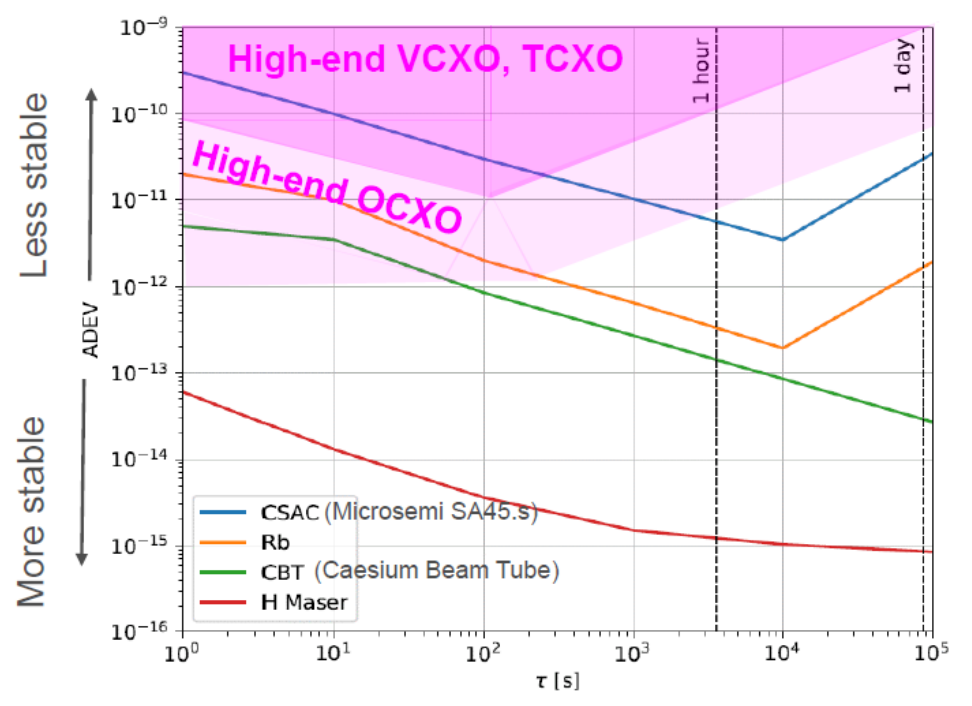
\includegraphics[width=0.8\textwidth]{img/allan_diagram}
        \caption{ADEV for traditional MEMS resonator vs. CSAC vs. full size atomic clock \cite{JRC-Tecnical-Report-1}}
    \end{figure}
\end{frame}



\begin{frame}{Temperature Sensitivity (Diagram)}
    \begin{figure}
        \centering
        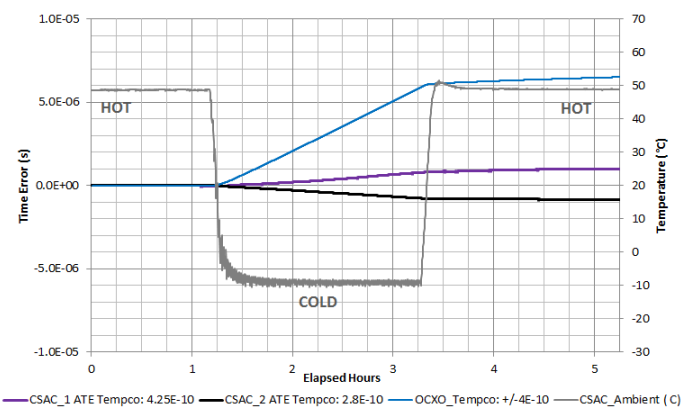
\includegraphics[width=0.9\textwidth]{img/temperature_deviation_effect}
        \caption{Temperature effect for traditional MEMS resonator vs. CSAC \cite{Microsemi-Temperature-Sentivity}}
    \end{figure}
\end{frame}



\begin{frame}[allowframebreaks]{References}
    \bibliography{ref}
    \bibliographystyle{abbrv}
\end{frame}



\end{document}